% Created by tikzDevice version 0.10.1 on 2018-01-17 15:27:33
% !TEX encoding = UTF-8 Unicode
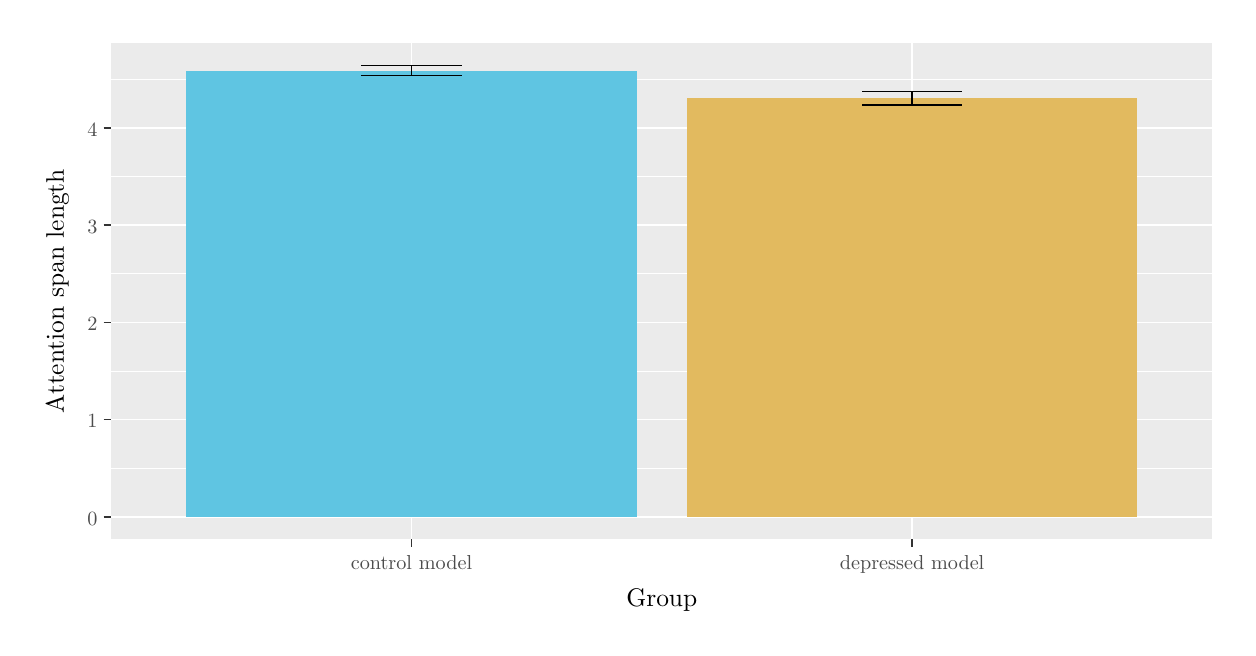
\begin{tikzpicture}[x=1pt,y=1pt]
\definecolor{fillColor}{RGB}{255,255,255}
\path[use as bounding box,fill=fillColor,fill opacity=0.00] (0,0) rectangle (433.62,216.81);
\begin{scope}
\path[clip] (  0.00,  0.00) rectangle (433.62,216.81);
\definecolor{drawColor}{RGB}{255,255,255}
\definecolor{fillColor}{RGB}{255,255,255}

\path[draw=drawColor,line width= 0.6pt,line join=round,line cap=round,fill=fillColor] (  0.00,  0.00) rectangle (433.62,216.81);
\end{scope}
\begin{scope}
\path[clip] ( 30.17, 31.92) rectangle (428.12,211.31);
\definecolor{fillColor}{gray}{0.92}

\path[fill=fillColor] ( 30.17, 31.92) rectangle (428.12,211.31);
\definecolor{drawColor}{RGB}{255,255,255}

\path[draw=drawColor,line width= 0.3pt,line join=round] ( 30.17, 57.63) --
	(428.12, 57.63);

\path[draw=drawColor,line width= 0.3pt,line join=round] ( 30.17, 92.74) --
	(428.12, 92.74);

\path[draw=drawColor,line width= 0.3pt,line join=round] ( 30.17,127.86) --
	(428.12,127.86);

\path[draw=drawColor,line width= 0.3pt,line join=round] ( 30.17,162.97) --
	(428.12,162.97);

\path[draw=drawColor,line width= 0.3pt,line join=round] ( 30.17,198.08) --
	(428.12,198.08);

\path[draw=drawColor,line width= 0.6pt,line join=round] ( 30.17, 40.07) --
	(428.12, 40.07);

\path[draw=drawColor,line width= 0.6pt,line join=round] ( 30.17, 75.19) --
	(428.12, 75.19);

\path[draw=drawColor,line width= 0.6pt,line join=round] ( 30.17,110.30) --
	(428.12,110.30);

\path[draw=drawColor,line width= 0.6pt,line join=round] ( 30.17,145.41) --
	(428.12,145.41);

\path[draw=drawColor,line width= 0.6pt,line join=round] ( 30.17,180.53) --
	(428.12,180.53);

\path[draw=drawColor,line width= 0.6pt,line join=round] (138.70, 31.92) --
	(138.70,211.31);

\path[draw=drawColor,line width= 0.6pt,line join=round] (319.59, 31.92) --
	(319.59,211.31);
\definecolor{fillColor}{RGB}{95,197,226}

\path[fill=fillColor] ( 57.30, 40.07) rectangle (220.10,201.33);
\definecolor{fillColor}{RGB}{226,186,95}

\path[fill=fillColor] (238.19, 40.07) rectangle (400.99,191.34);
\definecolor{drawColor}{RGB}{0,0,0}

\path[draw=drawColor,line width= 0.6pt,line join=round] (120.61,203.16) --
	(156.79,203.16);

\path[draw=drawColor,line width= 0.6pt,line join=round] (138.70,203.16) --
	(138.70,199.50);

\path[draw=drawColor,line width= 0.6pt,line join=round] (120.61,199.50) --
	(156.79,199.50);

\path[draw=drawColor,line width= 0.6pt,line join=round] (301.50,193.70) --
	(337.68,193.70);

\path[draw=drawColor,line width= 0.6pt,line join=round] (319.59,193.70) --
	(319.59,188.98);

\path[draw=drawColor,line width= 0.6pt,line join=round] (301.50,188.98) --
	(337.68,188.98);
\end{scope}
\begin{scope}
\path[clip] (  0.00,  0.00) rectangle (433.62,216.81);
\definecolor{drawColor}{gray}{0.30}

\node[text=drawColor,anchor=base east,inner sep=0pt, outer sep=0pt, scale=  0.73] at ( 25.22, 37.04) {0};

\node[text=drawColor,anchor=base east,inner sep=0pt, outer sep=0pt, scale=  0.73] at ( 25.22, 72.16) {1};

\node[text=drawColor,anchor=base east,inner sep=0pt, outer sep=0pt, scale=  0.73] at ( 25.22,107.27) {2};

\node[text=drawColor,anchor=base east,inner sep=0pt, outer sep=0pt, scale=  0.73] at ( 25.22,142.38) {3};

\node[text=drawColor,anchor=base east,inner sep=0pt, outer sep=0pt, scale=  0.73] at ( 25.22,177.50) {4};
\end{scope}
\begin{scope}
\path[clip] (  0.00,  0.00) rectangle (433.62,216.81);
\definecolor{drawColor}{gray}{0.20}

\path[draw=drawColor,line width= 0.6pt,line join=round] ( 27.42, 40.07) --
	( 30.17, 40.07);

\path[draw=drawColor,line width= 0.6pt,line join=round] ( 27.42, 75.19) --
	( 30.17, 75.19);

\path[draw=drawColor,line width= 0.6pt,line join=round] ( 27.42,110.30) --
	( 30.17,110.30);

\path[draw=drawColor,line width= 0.6pt,line join=round] ( 27.42,145.41) --
	( 30.17,145.41);

\path[draw=drawColor,line width= 0.6pt,line join=round] ( 27.42,180.53) --
	( 30.17,180.53);
\end{scope}
\begin{scope}
\path[clip] (  0.00,  0.00) rectangle (433.62,216.81);
\definecolor{drawColor}{gray}{0.20}

\path[draw=drawColor,line width= 0.6pt,line join=round] (138.70, 29.17) --
	(138.70, 31.92);

\path[draw=drawColor,line width= 0.6pt,line join=round] (319.59, 29.17) --
	(319.59, 31.92);
\end{scope}
\begin{scope}
\path[clip] (  0.00,  0.00) rectangle (433.62,216.81);
\definecolor{drawColor}{gray}{0.30}

\node[text=drawColor,anchor=base,inner sep=0pt, outer sep=0pt, scale=  0.73] at (138.70, 20.91) {control model};

\node[text=drawColor,anchor=base,inner sep=0pt, outer sep=0pt, scale=  0.73] at (319.59, 20.91) {depressed model};
\end{scope}
\begin{scope}
\path[clip] (  0.00,  0.00) rectangle (433.62,216.81);
\definecolor{drawColor}{RGB}{0,0,0}

\node[text=drawColor,anchor=base,inner sep=0pt, outer sep=0pt, scale=  0.92] at (229.14,  7.83) {Group};
\end{scope}
\begin{scope}
\path[clip] (  0.00,  0.00) rectangle (433.62,216.81);
\definecolor{drawColor}{RGB}{0,0,0}

\node[text=drawColor,rotate= 90.00,anchor=base,inner sep=0pt, outer sep=0pt, scale=  0.92] at ( 13.08,121.61) {Attention span length};
\end{scope}
\end{tikzpicture}
